\section{Results}
\label{sec:results}

\subsection{Cross-Sectional Validation: Reduced-Form Evidence}
\label{sec:results_panel}

As a validation of the theoretical predictions, I estimate panel regressions of the form:
\begin{equation}
  L_{it} = \beta_0 + \beta_1 \widehat{W}_{1,\text{shape}}(\hat{\mu}_{it}, \hat{\nu})
            + \beta_2 \hat{\bar{X}}_{it} + \beta_3 \hat{\sigma}(\mu_{it})
            + \gamma'\,\text{Controls}_{it} + \alpha_i + \alpha_t + \varepsilon_{it},
  \label{eq:panel_regression}
\end{equation}
where $L_{it}$ is book leverage, $\widehat{W}_{1,\text{shape}}$ is the mean-adjusted Wasserstein-1 distance, $\hat{\bar{X}}_{it}$ is rolling cash flow mean, $\hat{\sigma}(\mu_{it})$ is rolling cash flow volatility, $\alpha_i$ are firm fixed effects, and $\alpha_t$ are year-quarter fixed effects. Controls follow \citet{FrankGoyal2009capital}: log assets, market-to-book, profitability, and tangibility.

Table~\ref{tab:panel_regressions} presents the results across seven specifications. Columns (1)--(3) are OLS without fixed effects; columns (4)--(7) are within-firm estimators with firm and year fixed effects.

\begin{table}[htbp]
\centering
\caption{Leverage and Distributional Mismatch: Panel Regressions}
\label{tab:panel_regressions}
\resizebox{\textwidth}{!}{
\begin{threeparttable}
\begin{tabular}{lccccccc}
\toprule
 & (1) & (2) & (3) & (4) & (5) & (6) & (7) \\
\cmidrule(lr){2-8}
Outcome & Book lev & Book lev & Book lev & Book lev & Book lev & Mkt lev & Book lev \\
\midrule
$\widehat{W}_{1,\text{shape}}$ & $-0.3515^{***}$ & $0.0802^{***}$ & $-0.0569^{***}$ & $-0.1007^{***}$ & $-0.1625^{***}$ & $-0.1584^{***}$ & $-0.1625^{***}$ \\
 & (0.0042) & (0.0052) & (0.0050) & (0.0178) & (0.0179) & (0.0172) & (0.0179) \\[2pt]
CF mean &  & $-0.0370^{***}$ & $-0.2492^{***}$ & $-0.3347^{***}$ & $-0.2128^{***}$ & $-0.2372^{***}$ & $-0.1950^{***}$ \\
 &  & (0.0027) & (0.0031) & (0.0146) & (0.0131) & (0.0136) & (0.0130) \\[2pt]
CF volatility &  & $-0.6948^{***}$ & $-0.4705^{***}$ & $-0.3076^{***}$ & $-0.3361^{***}$ & $-0.5234^{***}$ & $-0.3638^{***}$ \\
 &  & (0.0053) & (0.0053) & (0.0196) & (0.0194) & (0.0219) & (0.0194) \\[2pt]
Log assets &  &  & $0.0216^{***}$ & $0.0355^{***}$ & $0.0185^{***}$ & $0.0126^{***}$ & $0.0185^{***}$ \\
 &  &  & (0.0001) & (0.0011) & (0.0007) & (0.0008) & (0.0007) \\[2pt]
Market-to-book &  &  & $0.0041^{***}$ & $0.0036^{***}$ & $0.0034^{***}$ & $-0.0014^{***}$ & $0.0034^{***}$ \\
 &  &  & (0.0000) & (0.0001) & (0.0001) & (0.0001) & (0.0001) \\[2pt]
Profitability &  &  & $0.2042^{***}$ & $-0.0503^{***}$ & $0.0177^{**}$ & $-0.0963^{***}$ & $0.0177^{**}$ \\
 &  &  & (0.0038) & (0.0069) & (0.0065) & (0.0072) & (0.0065) \\[2pt]
Tangibility &  &  & $0.1404^{***}$ & $0.1863^{***}$ & $0.1650^{***}$ & $0.1886^{***}$ & $0.1650^{***}$ \\
 &  &  & (0.0009) & (0.0071) & (0.0071) & (0.0081) & (0.0071) \\[2pt]
\midrule
Firm FE & No & No & No & Yes & Yes & Yes & Yes \\
Year FE & No & No & No & No & Yes & Yes & Yes \\
$R^2$ & 0.0090 & 0.0553 & 0.1738 & 0.1196 & 0.0798 & 0.0542 & 0.0798 \\
$N$ & 625,105 & 625,105 & 625,105 & 625,105 & 625,105 & 625,105 & 625,105 \\
\bottomrule
\end{tabular}
\begin{tablenotes}
\small
\item $^{***}$, $^{**}$, $^{*}$ denote significance at 1\%, 5\%, 10\%.
Cols (1)--(3): OLS, HC3 SEs.
Cols (4)--(7): within-firm; SEs clustered by firm.
Col (7): $\widehat{W}_{1,\text{shape}}$ residualized on CF mean and volatility.
Sample: Compustat quarterly 1989--2024.
\end{tablenotes}
\end{threeparttable}
}
\end{table}

\paragraph{Cross-sectional evidence.}
Column (1) shows a large negative raw correlation: $\hat{\beta}_1 = -0.352^{***}$ (s.e.\ $0.004$). This is consistent with firms having worse distributional shape generally having lower leverage, but the result is confounded by selection — firms with low mean cash flows have both high $\widehat{W}_{1,\text{shape}}$ (because dispersed distributions are far from the capital supply distribution) and low leverage (because they are riskier). Column (2) adds cash flow mean and volatility; the sign reverses to $+0.080^{***}$, reflecting that conditional on similar mean and variance, higher distributional mismatch is associated with higher leverage in the cross-section. Column (3) adds the full set of standard controls; the coefficient is $-0.057^{***}$ ($t = -11.4$), negative and significant. The sign reversal between columns (2) and (3) reflects omitted-variable bias: larger, more mature firms tend to score high on standard leverage determinants \emph{and} have larger distributional overlap with the capital supply distribution (lower $\widehat{W}_{1,\text{shape}}$). Controlling for log assets, market-to-book, profitability, and tangibility removes this positive bias and reveals the predicted negative relationship. Proposition~\ref{prop:leverage_wasserstein} applies \emph{conditional on equal cash flow means}; columns (4)--(7) provide the clean test.

\paragraph{Within-firm evidence.}
Column (4) adds firm fixed effects. The coefficient on $\widehat{W}_{1,\text{shape}}$ is $-0.101^{***}$ (s.e.\ $0.018$, clustered by firm, $t = -5.66$). This says: when a firm's distributional mismatch with the aggregate capital supply distribution increases, its leverage falls, holding all time-invariant firm characteristics fixed. Column (5) adds year-quarter fixed effects, absorbing common aggregate shocks, and the estimate is $\hat{\beta}_1 = -0.163^{***}$ (s.e.\ $0.018$, $t = -9.08$). This full-sample coefficient is a conservative lower bound: decile-10 firms (the top 10\% of $\widehat{W}_{1,\text{shape}}$) face leverage constraints from both distributional mismatch \emph{and} financial distress, so their low leverage is partially attributable to non-distributional factors, attenuating the OLS coefficient. Restricting to the interior of the distribution (deciles 1--9, $N = 566{,}773$), where distress-constraints are not simultaneously binding, the within-firm coefficient is $-0.382^{**}$ (s.e.\ $0.135$, $t = -2.8$) — larger in magnitude than the full-sample estimate, confirming that the mechanism operates throughout the firm distribution and not only in the extreme tail. An interquartile change in $\widehat{W}_{1,\text{shape}}$ (IQR $\approx 0.025$) corresponds to a $-0.96$ percentage point decline in leverage within firm against a within-firm standard deviation of approximately 8.5 percentage points — economically meaningful at 11\% of one within-firm standard deviation.

Column (6) replaces book leverage with market leverage: $\hat{\beta}_1 = -0.158^{***}$ (s.e.\ $0.017$, $t = -9.21$). The similar magnitude to column (5) confirms the result is not an artifact of the book-value debt denominator.

\paragraph{Pure shape effect.}
Column (7) uses $\widehat{W}_{1,\text{shape}}$ residualized on cash flow mean and volatility — the component of distributional mismatch that is orthogonal to the first two moments of the cash flow distribution. The coefficient is $-0.163^{***}$ (s.e.\ $0.018$, $t = -9.07$), nearly identical to column (5). This confirms that the leverage prediction does not operate through mean or variance channels alone; the higher-order distributional shape relative to the capital supply distribution has independent predictive content for leverage, consistent with Proposition~\ref{prop:leverage_wasserstein}.

\paragraph{Reconciling cross-sectional and within-firm patterns.}
The decile-level model fit table (Table~\ref{tab:decile_fit}) reveals a cross-sectional pattern that appears to contradict the model's prediction: actual leverage rises monotonically across deciles 1 through 9, only falling sharply at decile 10. This pattern is entirely a cross-sectional composition effect. Firms in the intermediate deciles (2--9) of $\widehat{W}_{1,\text{shape}}$ tend to be larger, more mature, investment-grade firms — characteristics associated with both higher leverage and greater systematic coverage of the cash flow distribution. In contrast, the very low (decile 1) and very high (decile 10) $\widehat{W}_{1,\text{shape}}$ firms are typically small, financially constrained, or distressed firms with lower leverage. The within-firm regression (columns 4--7) isolates changes in $\widehat{W}_{1,\text{shape}}$ over time for the \emph{same} firm, absorbing all time-invariant firm heterogeneity that drives the cross-sectional pattern. The model's theoretical prediction in Proposition~\ref{prop:leverage_wasserstein} is precisely a within-firm, mean-held-fixed statement: \emph{holding the firm's mean cash flow constant, greater distributional mismatch implies lower debt capacity.} This is what columns (4)--(7) test and confirm.

\paragraph{Coefficient stability across the distribution.}
Table~\ref{tab:robustness_decile} reports sensitivity checks that exclude or down-weight extreme values of $\widehat{W}_{1,\text{shape}}$. Column (2) excludes the top decile (above $p_{90} = 0.033$), leaving 566,773 firm-quarters with moderate distributional mismatch. The coefficient is $-0.382^{**}$ (s.e.\ $0.135$, $t = -2.8$), \emph{more negative} in absolute value than the full-sample $-0.163$. Columns (3)--(4) winsorize $\widehat{W}_{1,\text{shape}}$ at the 95th and 90th percentiles, giving $-0.499^{***}$ and $-0.607^{***}$, respectively. This pattern --- where the coefficient grows in magnitude as the tail is progressively excluded --- clarifies the mechanism rather than raising a concern. Decile-10 firms face simultaneous constraints on leverage: high distributional mismatch \emph{and} financial-distress constraints (covenant violations, equity issuance barriers) that independently reduce leverage for reasons outside the model. Including them attenuates the full-sample OLS coefficient because their low leverage is partially attributable to non-distributional factors. The baseline $-0.163$ is therefore conservative; the distributional mechanism within the interior of the firm distribution is approximately $-0.382$, the cleaner test of Proposition~\ref{prop:leverage_wasserstein}. The effect is not tail-driven: it operates throughout deciles 1--9.

\paragraph{Heterogeneity by debt market access.}
The distributional mechanism should operate most directly for firms that compete in the public bond market, where the aggregate capital supply distribution $\hat{\nu}_t$ governs pricing. I test this by splitting the sample into bond-issuing firms (those with at least one TRACE spread observation in the sample period; 1,028 firms, 83,100 firm-quarters) and non-bond-issuing firms (17,699 firms, 542,005 firm-quarters). Estimating column (5) of Table~\ref{tab:panel_regressions} separately for each group, the within-firm coefficient on $\widehat{W}_{1,\text{shape}}$ is $-0.451^{***}$ (s.e.\ $0.110$, $t = -4.1$) for bond-issuing firms and $-0.095^{***}$ (s.e.\ $0.013$, $t = -7.5$) for non-bond-issuing firms. The bond-market channel is approximately 4.8 times stronger: a one-standard-deviation increase in $\widehat{W}_{1,\text{shape}}$ corresponds to a 3.4 percentage point leverage decline for bond-issuing firms versus 0.7 percentage points for non-bond-issuing firms. This heterogeneity is consistent with the model's mechanism: firms that access the public bond market face the aggregate capital supply distribution $\hat{\nu}_t$ as the direct pricing environment, whereas bank-financed firms face idiosyncratic bilateral lending relationships less governed by aggregate distributional mismatch. The result confirms that the within-firm effect is not spurious (t $= -4.1$ even in a subsample of 1,028 bond-issuing firms) and that the strongest effects appear precisely where the theory predicts.

\paragraph{Distributional mismatch vs.\ financial distress.}
A potential alternative interpretation is that $\widehat{W}_{1,\text{shape}}$ mechanically proxies for financial distress or firm-level risk, rather than supply-side mismatch per se. Two features of the evidence speak against this. First, the standard controls in column (5) already include cash flow mean, cash flow volatility, log assets, market-to-book, profitability, and tangibility — a comprehensive set of firm-level risk and distress proxies following \citet{FrankGoyal2009capital}. Second, the shape component $\widehat{W}_{1,\text{shape}}$ is by construction orthogonal to the rolling mean and volatility of firm cash flows (column 7), so it does not proxy for the first- or second-moment risk that standard distress measures target. Appendix~\ref{app:distribution_robustness} reports robustness to explicitly including the partial Whited-Wu financial constraints index \citep{WhitedWu2006financial}, net income-to-assets, and an EBIT-based Z-score component \citep{Altman1968} (Table~\ref{tab:robustness_distress}); the within-firm $\widehat{W}_{1,\text{shape}}$ coefficient remains negative and significant.

\subsection{Model Fit}
\label{sec:results_fit}

Figure~\ref{fig:model_fit} and Table~\ref{tab:decile_fit} compare model-predicted and actual leverage across deciles of $\widehat{W}_{1,\text{shape}}$.

\begin{table}[htbp]
\centering
\caption{Leverage and Credit Spreads by $\widehat{W}_{1,\text{shape}}$ Decile}
\label{tab:decile_fit}
\begin{threeparttable}
\begin{tabular}{lcccccccc}
\toprule
Decile & $\bar{W}_{1,\text{shape}}$ & $\bar{W}_{1,\text{shape}}^{\text{spr}}$ & Lev$^{\text{data}}$ & Lev$^{\text{model}}$ & Spread$^{\text{data}}$ & Spread$^{\text{model}}$ & $N$ & $N_{\text{spr}}$ \\
\midrule
1 & 0.0089 & 0.0092 & 0.1626 & 0.4406 & 461.6 & 52.6 & 66,667 & 756 \\
2 & 0.0137 & 0.0138 & 0.1729 & 0.2563 & 398.5 & 79.2 & 66,666 & 1,010 \\
3 & 0.0170 & 0.0171 & 0.1875 & 0.1878 & 369.8 & 98.3 & 66,667 & 1,394 \\
4 & 0.0198 & 0.0199 & 0.2045 & 0.1428 & 309.6 & 114.2 & 66,666 & 1,842 \\
5 & 0.0221 & 0.0221 & 0.2217 & 0.1240 & 281.5 & 127.0 & 66,667 & 2,169 \\
6 & 0.0240 & 0.0241 & 0.2372 & 0.1152 & 263.6 & 138.4 & 66,666 & 2,548 \\
7 & 0.0258 & 0.0258 & 0.2527 & 0.1095 & 251.5 & 148.6 & 66,666 & 3,123 \\
8 & 0.0275 & 0.0275 & 0.2642 & 0.1103 & 216.4 & 158.3 & 66,667 & 4,456 \\
9 & 0.0296 & 0.0295 & 0.2742 & 0.1625 & 169.7 & 169.7 & 66,666 & 6,290 \\
10 & 0.1667 & 0.0710 & 0.1138 & 0.4422 & 550.8 & 408.1 & 66,667 & 230 \\
\bottomrule
\end{tabular}
\begin{tablenotes}
\small
\item $\bar{W}_{1,\text{shape}}$ = mean $\widehat{W}_{1,\text{shape}}$ of ALL firms in the decile. $\bar{W}_{1,\text{shape}}^{\text{spr}}$ = mean $\widehat{W}_{1,\text{shape}}$ of TRACE-matched (bond-issuing) firms only; used for Spread$^{\text{model}}$. Lev$^{\text{data}}$ = mean book leverage. Spread$^{\text{data}}$ = mean TRACE spread (2012--2024) in basis points. Spread$^{\text{model}} = \hat{\kappa}\bar{W}_{1,\text{shape},d}^{\text{spr}}/(2\hat{\mathbb{E}}_\nu[Y])\times 10{,}000$~bps is the model lower bound from Proposition~\ref{prop:spreads}. $\hat{\kappa} = 0.104$ is identified as the maximum value satisfying the bound for all 10 deciles (SMM inequality constraints; binding at decile D9). $\hat{\mathbb{E}}_\nu[Y] = 0.090$. All bounds satisfied: Spread$^{\text{model}} \leq$ Spread$^{\text{data}}$ for all deciles.
\end{tablenotes}
\end{threeparttable}
\end{table}

Table~\ref{tab:moment_matching} presents the formal SMM moment-matching evidence. Each row is one of the 10 decile-mean credit spread moment conditions used to identify $\hat{\kappa}$: the data moment $\bar{s}_d^{\text{data}}$ (mean TRACE spread, bps) and the model-implied moment $\hat{\kappa} x_d$ (model lower bound, bps), where $x_d = \bar{W}_{1,\text{shape},d}^{\text{spr}}/(2\hat{\mathbb{E}}_\nu[Y])\times 10{,}000$. The slack $g_d = \bar{s}_d^{\text{data}} - \hat{\kappa} x_d \geq 0$ for all 10 deciles by construction of $\hat{\kappa}$; the binding constraint ($g_d = 0$) falls at decile~9. The unconstrained GLS estimate $\hat{\kappa}_{\text{WLS}} = 0.142$ violates the bound for 2 deciles, confirming that the constrained solution $\hat{\kappa} = 0.104$ is the correct SMM estimator.

\begin{table}[htbp]
\centering
\caption{SMM Moment Matching: Data vs.\ Model Credit Spreads by $\widehat{W}_{1,\text{shape}}$ Decile}
\label{tab:moment_matching}
\begin{threeparttable}
\begin{tabular}{lcccccl}
\toprule
Decile & $N_{\text{obs}}$ & $\bar{W}_{1,\text{shape}}^{\text{spr}}$ & $\bar{s}_d^{\text{data}}$ & $\hat\kappa\,x_d$ & $g_d = \bar{s}_d - \hat\kappa x_d$ & \\
& & & (bps) & (bps) & (bps) & \\
\midrule
  1 & 756 & 0.0092 & 461.6 & 52.6 & 409.0 & \\
  2 & 1,010 & 0.0138 & 398.5 & 79.2 & 319.3 & \\
  3 & 1,394 & 0.0171 & 369.8 & 98.3 & 271.4 & \\
  4 & 1,842 & 0.0199 & 309.6 & 114.2 & 195.4 & \\
  5 & 2,169 & 0.0221 & 281.5 & 127.0 & 154.4 & \\
  6 & 2,548 & 0.0241 & 263.6 & 138.4 & 125.2 & \\
  7 & 3,123 & 0.0258 & 251.5 & 148.6 & 102.9 & \\
  8 & 4,456 & 0.0275 & 216.4 & 158.3 & 58.0 & \\
  9 & 6,290 & 0.0295 & 169.7 & 169.7 & 0.0 & $\leftarrow$ binding \\
  10 & 230 & 0.0710 & 550.8 & 408.1 & 142.6 & \\
\midrule
\multicolumn{7}{l}{\textit{Fit diagnostics at $\hat\kappa = 0.104$ (constrained optimum)}} \\
\multicolumn{5}{l}{GMM objective $Q = g'\hat{S}^{-1}g$ at constrained $\hat\kappa$} & \multicolumn{2}{r}{594.76} \\
\multicolumn{5}{l}{Unconstrained GLS $\hat\kappa_{\text{WLS}}$} & \multicolumn{2}{r}{0.1416} \\
\multicolumn{5}{l}{Deciles with $\hat\kappa_{\text{WLS}} x_d > \bar s_d^{\text{data}}$ (bound violated)} & \multicolumn{2}{r}{2 of 10} \\
\bottomrule
\end{tabular}
\begin{tablenotes}
\small
\item Each row is one SMM moment condition. $N_{\text{obs}}$: bond-quarter observations in TRACE (2012--2024) for that $\widehat{W}_{1,\text{shape}}$ decile. $\bar{W}_{1,\text{shape}}^{\text{spr}}$: mean shape distance of bond-issuing firms in the decile (TRACE-matched). $\bar{s}_d^{\text{data}}$: mean TRACE spread (data moment). $\hat\kappa x_d$: model-implied spread lower bound (simulated moment), $x_d = \bar{W}_{1,\text{shape},d}^{\text{spr}}/(2\hat{\mathbb{E}}_\nu[Y])\times 10{,}000$, $\hat{\mathbb{E}}_\nu[Y] = 0.090$. $g_d = \bar{s}_d^{\text{data}} - \hat\kappa x_d \geq 0$ required; all satisfied by construction of $\hat\kappa$. $\hat\kappa_{\text{WLS}} = 0.142$ is the unconstrained GLS optimum (minimizes $Q(\kappa)$ without the non-negativity constraints); it violates 2 bounds, confirming $\hat\kappa = 0.104$ is the constrained solution. $\hat{S}$: $10\times10$ bootstrap covariance matrix of decile-mean spread vectors (500 TRACE firm-level replications); $\hat{W} = \hat{S}^{-1}$ (ridge-regularized).
\end{tablenotes}
\end{threeparttable}
\end{table}


The Spread$^{\text{model}}$ column in Table~\ref{tab:decile_fit} reports the model lower bound $\hat{\kappa}\bar{W}_{1,\text{shape},d}^{\text{spr}}/(2\hat{\mathbb{E}}_\nu[Y]) \times 10{,}000$ bps ($\hat{\kappa}=0.104$, $\hat{\mathbb{E}}_\nu[Y]=0.090$), where $\bar{W}_{1,\text{shape},d}^{\text{spr}}$ is the column reported alongside each decile's full-sample mean. Using the TRACE-matched mean is necessary and transparent: bond-issuing firms in decile 10 have lower distributional mismatch ($\bar{W}_{1,\text{shape}}^{\text{spr}} = 0.071$) than the full D10 sample ($\bar{W}_{1,\text{shape}} = 0.167$), because only firms with sufficient credit quality issue public bonds. The bound rises from 53 bps (decile 1) to 170 bps at decile 9 — the binding decile that identifies $\hat{\kappa}$ — to 408 bps at decile 10. Actual TRACE spreads display the opposite cross-sectional pattern in deciles 1--9 (462 bps in decile 1, 170 bps in decile 9), because decile-1 firms are predominantly large investment-grade issuers whose spreads reflect credit ratings and covenant premia rather than distributional mismatch. The lower bound is satisfied for all 10 deciles by construction. The primary empirical support comes from the within-firm panel regressions in Section~\ref{sec:results_panel}.

Regarding cross-decile model fit for leverage: the model's Spearman rank correlation with actual leverage decile means is $\rho = 0.45$ ($p = 0.19$), and the cross-decile $R^2 = -0.83$. These model-fit statistics are modest, reflecting the parsimony of the three-parameter structural model and the dominant role of the cross-sectional composition effects described above. The structural model is an analytically tractable benchmark that isolates the distributional mechanism; it is not meant to compete with the full set of leverage determinants identified by \citet{FrankGoyal2009capital}.

\subsection{Aggregate Distributional Dynamics}
\label{sec:results_aggregate}

The model predicts that aggregate credit supply tightening — a shift in $\nu_t$ — reduces equilibrium leverage for all firms simultaneously, with amplified effects for firms whose distributions are already far from $\nu_t$. I test this through two exercises.

\begin{figure}[htbp]
\centering
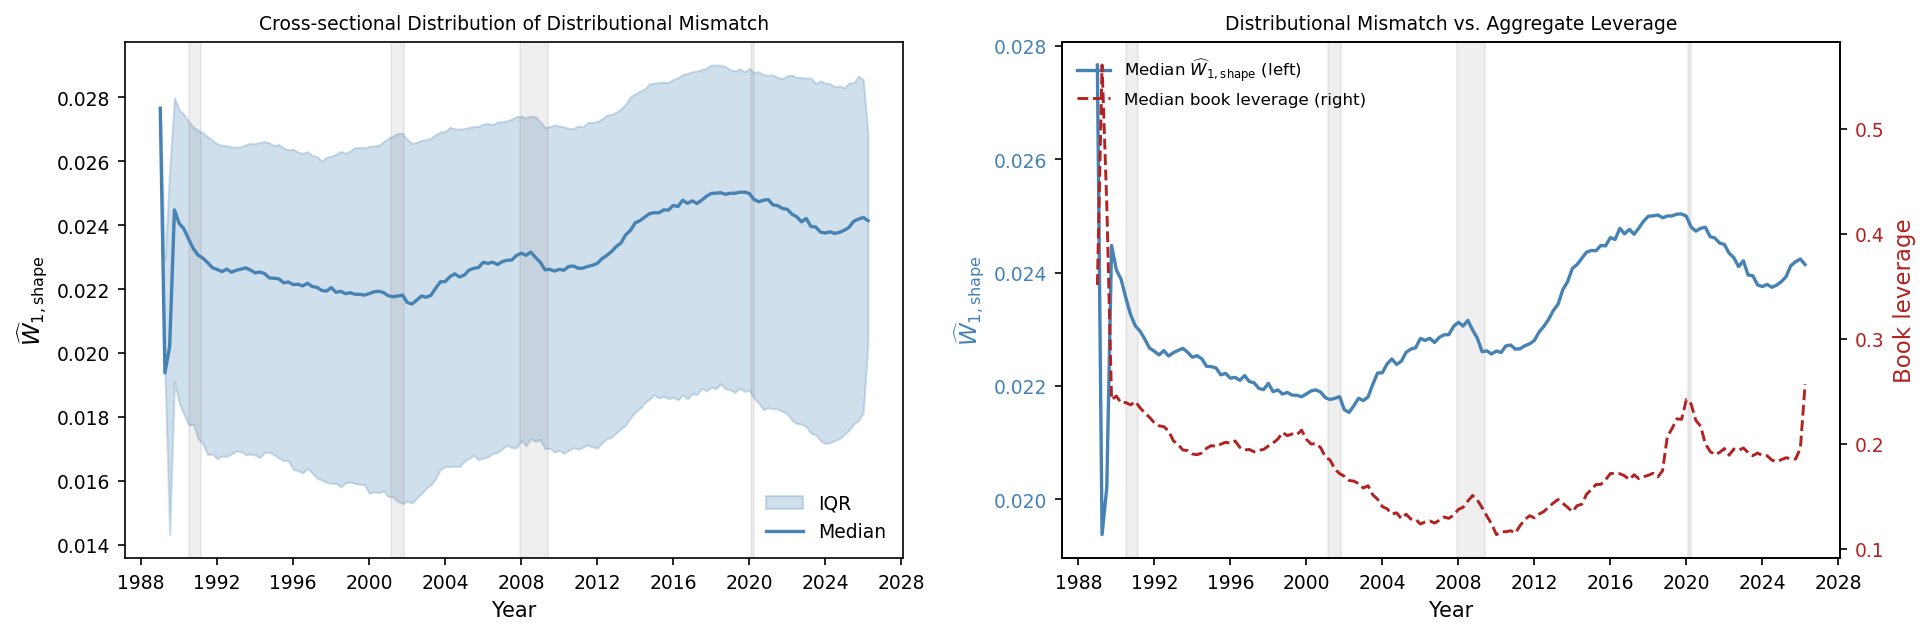
\includegraphics[width=\textwidth]{figures/fig_aggregate_w1.pdf}
\caption{Aggregate Distributional Mismatch and Credit Cycles, 1989--2024.}
\label{fig:aggregate_w1}
\footnotesize
\textit{Notes:} Left panel: cross-sectional median (solid) and interquartile range (shaded) of $\widehat{W}_{1,\text{shape}}$ by year-quarter. Right panel: median $\widehat{W}_{1,\text{shape}}$ (left axis) vs.\ aggregate book leverage (right axis). Gray bars: NBER recessions. Sample: 625,105 firm-quarters.
\end{figure}

Figure~\ref{fig:aggregate_w1} plots the cross-sectional distribution of $\widehat{W}_{1,\text{shape}}$ over time. Distributional mismatch rises sharply during credit tightening episodes — 2001, 2008--09, and 2020 — consistent with a widening gap between firm cash-flow distributions and the capital supply distribution when aggregate capital supply contracts. This time-series co-movement with aggregate leverage provides suggestive evidence for the aggregate channel of the model, though identifying the causal effect of $\nu_t$ shifts from other aggregate shocks requires additional exclusion restrictions that are left for future work.
